\documentclass{standalone}

\usepackage[margin=1in]{geometry}
\usepackage{tikz}
\usetikzlibrary{3d,calc}

\begin{document}

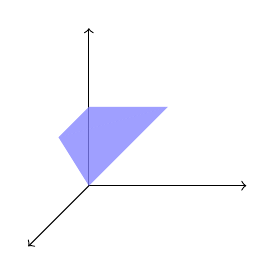
\begin{tikzpicture}
  \draw[->] (0, 0, 0) -- (2, 0, 0);
  \draw[->] (0, 0, 0) -- (0, 2, 0);
  \draw[->] (0, 0, 0) -- (0, 0, 2);

  \fill[blue!50,opacity=0.5] (0, 0, 0) -- (1, 1, 0) -- (0, 1, 0) -- (0, 0, 0);
  \fill[blue!50,opacity=0.5] (0, 0, 0) -- (1, 1, 0) -- (0, 1, 1) -- (0, 0, 0);
  \fill[blue!50,opacity=0.5] (0, 0, 0) -- (0, 1, 0) -- (0, 1, 1) -- (0, 0, 0);
  \fill[blue!50,opacity=0.5] (0, 1, 0) -- (1, 1, 0) -- (0, 1, 1) -- (0, 1, 0);
\end{tikzpicture}

\end{document}

%%% Local Variables:
%%% mode: latex
%%% TeX-master: t
%%% End:
